\documentclass[tikz,border=2pt]{standalone}
\usepackage{amsmath,amssymb}
\usepackage{tikz}
\usetikzlibrary{arrows.meta}

\begin{document}
% Inventory balance per month: I_{t-1} + P_t - d_t = I_t. Windows: month 1 demand 100,
% production 120 leaves 20 in stock; producing a month-3 window in month 2 costs 45 + 8
% holding versus 55 in month 3.
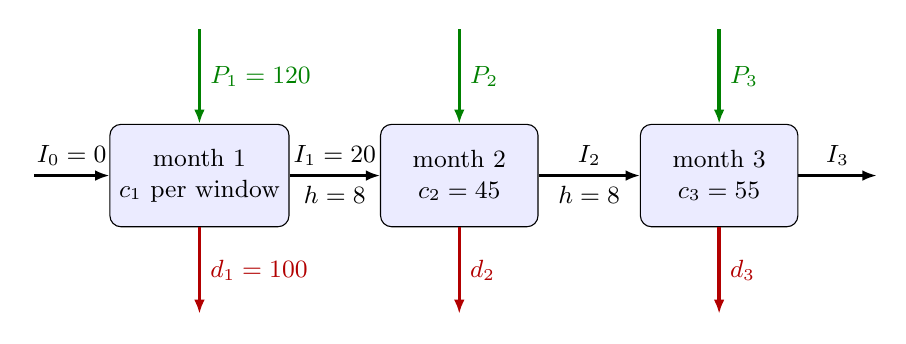
\begin{tikzpicture}[every node/.style={font=\small}, >={Latex[length=1.8mm]}, m/.style={draw, rounded corners=4pt, minimum width=2.0cm, minimum height=1.3cm, fill=blue!8, align=center}]
	\node[m] (m1) at (0,0) {month 1\\ $c_1$ per window};
	\node[m] (m2) at (3.3,0) {month 2\\ $c_2=45$};
	\node[m] (m3) at (6.6,0) {month 3\\ $c_3=55$};
	\foreach \n/\l in {m1/{$P_1=120$}, m2/{$P_2$}, m3/{$P_3$}} {\draw[->, green!50!black, very thick] ([yshift=1.2cm]\n.north) -- (\n.north) node[midway, right] {\l};}
	\foreach \n/\l in {m1/{$d_1=100$}, m2/{$d_2$}, m3/{$d_3$}} {\draw[->, red!70!black, very thick] (\n.south) -- ([yshift=-1.1cm]\n.south) node[midway, right] {\l};}
	\draw[->, thick] (-2.1,0) -- (m1) node[midway, above] {$I_0=0$};
	\draw[->, thick] (m1) -- (m2) node[midway, above] {$I_1=20$} node[midway, below] {$h=8$};
	\draw[->, thick] (m2) -- (m3) node[midway, above] {$I_2$} node[midway, below] {$h=8$};
	\draw[->, thick] (m3) -- (8.6,0) node[midway, above] {$I_3$};
	\end{tikzpicture}
\end{document}
